% This is a simple sample document.  For more complicated documents take a look in the exercise tab. Note that everything that comes after a % symbol is treated as comment and ignored when the code is compiled.

\documentclass{article} % \documentclass{} is the first command in any LaTeX code.  It is used to define what kind of document you are creating such as an article or a book, and begins the document preamble

\usepackage{amsmath} % \usepackage is a command that allows you to add functionality to your LaTeX code
\usepackage{authblk}
\usepackage{graphicx}

\title{A Foundation Model for RNA Velocity} % Sets article title
\author[1]{Josiah Bjorgaard} % Sets authors name
\affil[1]{Syntensor, Inc.}
\setcounter{Maxaffil}{0}
\renewcommand\Affilfont{\itshape\small}

\date{\today} % Sets date for date compiled

% The preamble ends with the command \begin{document}
\begin{document} % All begin commands must be paired with an end command somewhere
    \maketitle % creates title using information in preamble (title, author, date)
    
  \section{Abstract} % creates a section
    
  \section{Introduction}
Single cell foundation models make use of the total transcript reads per cell, effectively a measure of gene expression. Several foundation models also make use of additional single cell data modalities such as ATAC and surface protein abundance. In many scRNAseq experiments, the reads are able to be distinguished between spliced and unspliced transcripts. To date, this separation of RNAseq read counts has not been made useq of in single cell foundation models. It is an opportunity to use recent advances in multimodal transformers because it effectively presents the scRNASeq experiment as two well-aligned data modalities.

Recent advancements in foundation models and multimodal learning with transformers are able to be leveraged in order to train an embedding space which takes into account two or more modalities. These modalities can be of any form, but predominantly video, audio, and text. Foundation models based on LLMs are straightforwardly applied to sequential data, such as DNA and RNA sequence. Recently, foundation models for single cell data have also leveraged transformers to self-supervise on non-sequential (i.e. tabular) data comprised of gene expression and other sparse, continuous variables. These models can be used to fine tune to predictions related to the expression of genes, how gene expression defines cells, and infer the relationships between genes which define perturbation response.

RNA Velocity (RV) is a term denoting the rate of change of gene expression in a cell. It Is used to infer a cell's a trajectory in cellular state space, referred to as a pseudo-time trajectory. RV predictions are made using a single cell dataset (cell by gene matrices) of spliced and unspliced transcript counts which inform an ODE model of transcription, splicing, and degradation. The ODE model predictions of RV can be used to generate the pseudo-time series (ordering of cells according to their change in predicted gene expression), which effectively generates trajectories in cellular state space. Only a few studies have attempted to use deep learning to inform RV prediction and none to-date have attempted to build a single cell foundation model which can be applied to it.

The main sources of error in RV predictions are measurement noise and dropouts. Dropouts are responsible for the sparsity of measured genes in each cell. RV relies on interpolation schemes in order to make make use of sparsity in a single cell data. Although nearest neighbor interpolation is the predominant method for overcoming the sparsity in single cell data to allow RV prediction, it's accuracy is based on the density of samples in the cellular state space covered by a given dataset. The herein developed foundation model may improve these (TBD, to add to results).

The main contribution of this article are 
\begin{enumerate}
\setlength{\itemsep}{0pt}
\item the first single cell foundation model trained with spliced and unspliced transcript counts 
\item a data corpus of pre-processed scRNASeq data of spliced and unspliced transcript counts, freely released to the community
\item a fine-tuned model which can be used to predict RNA velocity from spliced/unspliced counts for any cell, without methods such as scVelo
\item a generative model for predicting cell state-space trajectories given a set of expression levels
\end{enumerate}

Importantly, the released model and model code can be used directly by single cell researchers to predict RV without existing ODE solver packages like scVelo, and to generatively produce pseudo-time trajectories from initial distributions of cell gene expression.

This article is organized as follows. First, related work is discussed. Second, the methods used to train the foundation model are described. Third, experiments which were carried out to pretrain the model and fine tune for RV prediction and other downstream tasks are detailed. Finally, discussion and future directions are described.

  \section{Related Work}
 Recent work has shown that MLMs are unable to reproduce the gene expression inputs and fail to integrate batch effects. In fact, scGPT produces only median gene expression values for any cell when not conditioned with cell embeddings. Both scGPT and geneformer predict well high expression genes when used as intended.\cite{kedzierska2023assessing}

  \subsection{Single Cell Foundation Models}
  \subsection{Deep RNA Velocity Models}
  \subsection{Multimodal Single Cell Models}
  \section{Methods}
  \subsection{Transformer Architecture}
The network architecture is derived from Zorro, a multimodal transformer with masked attention. Zorro allows both unimodal and multimodal inputs without representation collapse by using masked attention. Each modality undergoes self-attention, while cross attention occurs between modalities and a fusion representation. Outputs of the model are include unimodal, fusion, and global representation heads.

Zorro is trained with multimodal benchmarking datasets comprised of video, audio, and text modalities. In this model, we instead embed continuous RNA count measures for spliced and unspliced RNA as two separate modalities. Using the Zorro network architecture, we can include additional data modalities in the future.

  \subsubsection{Embeddings}
Positional encodings are required to give relational context to tokens in transformer architectures. In NLP, the encodings are crafted to provide information on the position of a token in a 1D sequence of tokens. On the contrary, in audio and video modalities for transformer architectures, the position embedding contains information on a patch location in 2D or frequency space (a patch embedding). The patch embedding is necessarily a linear projection of the 2D location of an image patch. The position encoding does not \textit{a priori}, need to provide information on the location of a token with respect to other tokens in the sequence. 

Single cell data is processed to a gene by cell matrix. Each cell is considered a sample. As discussed in previous section, single cell data is sparse, typically having data for 500-6000 genes per sample. This is compatible with existing transformer architectures, having a feasible sample length of 2048-16000 tokens per sample when using, e.g. flash attention. Larger sample lengths can be acheived using techniques such as Perceiver and HyENA. Models such as scGPT and scBERT use a fixed sample length which is simply the enumerated vocabulary of tokens, i.e. a list of all genes in the dataset, while adjusting the token embeddings to reflect the expression levels of the genes, which is the sole reason samples are differentiated. In contrast, models like Geneformer use a sequence of tokens reflecting the 

Single cell RNA measurements are groups non-sequential continuous variables, randomly selected in the measurement from a set of ~20k genes. While foundation models based on DNA and RNA sequences are his is fundamentally different from  sequential NLP tasks, and closer to embeddings generated for other modalities. 

In single cell data, most measurements can be matched with a gene. For spliced and unspliced transcripts, the embedding can be combined or separated. The vocabulary of ~18000 genes with an embedding size of 768 is ~13M parameters, which is multiplied by the number of modalities.
\subsubsection{Masked Attention}
\subsection{Training}
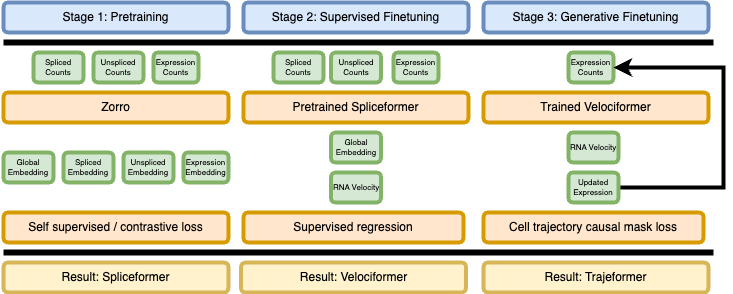
\includegraphics[scale=0.4]{fig1.drawio.png}
\subsubsection{Zorro fine tuning method}
We use the Adam optimiser with cosine
decay learning rate schedule, weight decay and learning rate
warmup. When fine-tuning, for Zorro-ViT and Zorro-Swin
we find better to use SGD optimiser and momentum 0.9. We
train all models for 50 epochs except for the ACAV-100M
datasets where we train for 10 epochs and the input-level and
bottleneck baselines where we train for 25 to prevent severe
overfitting. We find best to use nfusion = 6 in all models.
For AudioSet fine-tuning, we use mixup ($\alpha = 0.3$) and label
smoothing. We use cross-entropy loss for uni-label datasets
and binary sigmoid cross-entropy for multi-label. We train
one classifier for each of the 4 outputs of the model and
average its predictions. 
 \subsubsection{Contrastive Pre-Training}
An encoder was developed which learns the spliced, unspliced, and total RNA expression counts. This network architecture is based on the Zorro framework. 
\subsubsection{Expression Decoder}
We use supervised learning to train the pooling cross-attention layer to predict the expression of a gene using a separate genes embedding for the query. How does it perform cross-dataset?
\subsubsection{Velocity Decoder}
We use supervised learning to train the pooling cross-attention layer to predict the velocity of gene expression using separate gene embeddings for the query. How does it perform cross-dataset?
\subsubsection{Generative Decoder}
We use a generative MLM model with cross attention to generate the gene expression levels over pseudo-time.
Cell state-space include bifurcations and complex branching transitions between cell clusters, as well as potential cyclical transitions. \cite{van2020trajectory} Our approach is not intended to directly infer the topology of cell state space, but rather to determine the local direction and transitions that occur. Using generative gene expression to produce gene pseudo-time trajectories, we can produce a prediction of cell state space from combining multiple inferences.
Yet, we still must decide on a trajectory inference method. A comparison is given in
\cite{saelens2019comparison}
  \subsection{Data}
  \subsubsection{Data Sources}
  \subsubsection{Data Preprocessing}
Raw fastq files were downloaded from a variety of data sources. The fastq files were processed with the cellranger program to produce bam files. bam files were then processed with the Velocyto program in order to derive spliced and unspliced counts. The total dataset was filtered with scvelo using the $scvelo.pp.filter_and_normalize$ function, such that genes with < 1000 total counts were removed and cells with counts lower than 1000 were removed. The dataset was then processed using the datasets package into feather format. There are 36601 genes.
    \subsubsection{The RNA Velocity Corpus}
We have developed a large (30M cell) corpus of pre-processed scRNAseq experiments, comprised of single cell counts for spliced, unspliced, and ambiguous reads. This was prepared with the well-known Velocyto package. Included metadata provides a link to the experiment from which the counts are derived. This provides an opportunity for the single cell community to use the dataset to further develop multimodal foundation models with exisiting single cell data sources. The corpus size in feather format on disk is 20 TB.  \section{Results}

  \section{Discussion}
  
  \section{Acknolwedgments}
  Thanks to several people for useful discussions and potentially to AWS for support and Trainium usage.
 \section{References}
\bibliographystyle{unsrt}
\bibliography{references}

\end{document} % This is the end of the document